\documentclass[12pt,twoside]{article}

% La extensión total de la memoria deberá ser de un máximo de 50 páginas (excluidos resumen, índice y posibles anexos).

% Según las recomendaciones de estilo, el formato de la memoria se ajustará a lo siguiente:
% ? Formato del papel: DIN A4.
% ? Impresión a dos caras.
% ? Márgenes: superior e inferior, 2.5 cm. Márgenes laterales: páginas impares, izquierdo 4 cm y derecho 2 cm; páginas % pares, izquierdo 2 cm y derecho 4 cm.
% ? Tipo de letra: Times New Roman de 12 puntos.
% ? Interlineado: 1.5 líneas.
% ? Alineación: justificación completa.
% ? Sangrado de párrafo: 0.5 cm la primera línea de cada párrafo. No se
%pondrá espacio entre párrafos.
% ? Las páginas deberán ir numeradas en números arábigos.

% Teniendo en cuenta las indicaciones previas, definimos el estilo en LaTeX:

% Indicaciones para el idioma:
\usepackage[T1]{fontenc}
\usepackage[utf8]{inputenc}
\usepackage[spanish]{babel}

% Adaptación de itemize y enumerate a los usos tipograficos españoles:
\let\layoutspanish\relax
\addto\captionsspanish{\def\tablename{Tabla}} % para que escriba "Tabla" en lugar de "Cuadro"
\unaccentedoperators  % para que no acentúe los operadores

% Área de impresión de una página:
\usepackage[a4paper]{geometry}
  \geometry{hmargin={2.5cm,2.5cm},height=22cm}

% Formato de algunas distancias:
\renewcommand{\baselinestretch}{1.2}    % separación entre líneas de un mismo párrafo
\setlength{\partopsep}{0pt}
\setlength{\itemsep}{0pt}
\setlength{\topsep}{0pt}
\setlength{\parsep}{0pt}
\setlength{\parskip}{0.25\baselineskip}   % separación entre párrafos

\renewcommand{\textfraction}{0.1}   % mínima fracción de la página para el texto
\renewcommand{\topfraction}{1}      % máxima fracción de la página para objetos flotantes en la parte superior
\renewcommand{\bottomfraction}{1}
\renewcommand{\floatpagefraction}{1}

\setcounter{totalnumber}{5}
\setcounter{topnumber}{3}
\setcounter{bottomnumber}{2}

% Adaptación de las "caption" de los entorns "figure" y "table":
\usepackage{caption}
\setcaptionwidth{\textwidth}
\addtolength{\captionwidth}{-2\parindent}
\captionsetup{margin=\leftmargini,%
  width=\captionwidth,%
  labelfont={up,bf},%
  font={small,sl},%
  %indention={\captionindent
}

% Indentación del primer párrafo de una sección:
\usepackage{indentfirst}

% Definición del color grisclaro en la salida PDF:
\usepackage[pdftex]{color}

% Gráficos:
\usepackage[pdftex]{graphicx}

% Paquetes recomendados para la inclusión de fórmulas matemáticas:
\usepackage{amsmath}
\allowdisplaybreaks  % para que pueda partir fórmulas que ocupan más de una línea, necesita el paquete anterior
\usepackage{amssymb} % para cargar algunos símbolos como \blacksquare y \square
\usepackage{amsfonts} % para cargar algunas fuentes en estilo matemático
\usepackage{enumerate}
% Teoremas (se pueden definir todos los que se necesiten):


\newtheorem{theorem}{Teorema}[section]
\newtheorem{proposition}[theorem]{Proposición}
\newtheorem{definition}[theorem]{Definición}
\newtheorem{lemma}[theorem]{Lema}
\newtheorem{corollary}[theorem]{Corolario}
\newtheorem{example}[theorem]{Ejemplo}
\newtheorem{app}[theorem]{Aplicación}
\newtheorem{remark}[theorem]{Observación}
\newtheorem{agrad}[theorem]{Agradecimiento}
\newtheorem{algo}[theorem]{Algoritmo}
\newtheorem{axiom}[theorem]{Axioma}
\newtheorem{case}[theorem]{Caso}
\newtheorem{conclu}[theorem]{Conclusión}
\newtheorem{conjectura}[theorem]{Conjetura}
\newtheorem{notac}[theorem]{Notación}
\newtheorem{soluc}[theorem]{Solución}
\newtheorem{summary}[theorem]{Sumario}

\newtheorem{proof}[theorem]{Demostración.}
\renewenvironment{proof}{\textbf{\emph{Demostración.}}} {\quad \hfill $\blacksquare$ \newline} % para que aparezca un cuadrado negro al acabar la demostración


% Definición de cabeceras y pies de página:

\usepackage{fancyhdr}                     % para definir distintos tipos de cabeceras y pies de página

\newcommand{\RunningAuthor}{Adán Avilés Cahill}
\newcommand{\Author}[1]{\renewcommand{\RunningAuthor}{#1}}
\renewcommand{\leftmark}{\RunningAuthor}

\newcommand{\RunningTitle}{Hacking Ético}
\newcommand{\Title}[1]{\renewcommand{\RunningTitle}{#1}}
\renewcommand{\rightmark}{\RunningTitle}


\pagestyle{fancy}
\fancyhf{}
\fancyhead[LO]{\small \slshape \leftmark}    % lo que aparece en la parte izquierda de la páginas impares
\fancyhead[RE]{\small \slshape \rightmark}   % lo que aparece en la parte derecha de las páginas pares
\fancyhead[RO,LE]{\small \slshape \thepage}  % el número de página aparece en la parte exterior de la cabecera

\renewcommand{\headrulewidth}{0.6pt}         % grueso de la línea horizontal por debajo de la cabecera de la página
\renewcommand{\footrulewidth}{0pt}           % grueso de la línea horizontal por encima del pie de página
                                             % en este caso está vacío
\setlength{\headheight}{1.5\headheight}      % aumenta la altura de la cabecera en una parte y media

\fancypagestyle{plain}{%                     % redefinición del estilo de página 'plain'
  \fancyhf{}                                 % limpia todas las cabeceras y pies de página
  \setlength{\headwidth}{\textwidth}
  \fancyfoot[C]{\small \slshape \thepage}    % excepto el centro del pie de página
  \renewcommand{\headrulewidth}{0pt}
  \renewcommand{\footrulewidth}{0pt}
  }

% Instrucciones que se usan frecuentemente
\newcommand{\abs}[1]{\ensuremath{|#1|}}
\newcommand{\norm}[1]{\left\lVert#1\right\rVert} %norma
\newcommand{\normd}[1]{\left\lVert#1\right\rVert_{2}} %norma
\newcommand{\hil}{\mathcal{H} }
\newcommand{\prodes}[2]{\langle #1, #2 \rangle }
\newcommand{\suc}{\{x_n\}_{n=1}^{\infty}}
\newcommand{\sumi}[2]{\sum_{#1}^{#2}}
\newcommand{\luno}{L^1(\mathbb{R})}
\newcommand{\ldos}{L^2(\mathbb{R})}
\newcommand{\tf}[3]{\dfrac{1}{\sqrt{2 \pi}} \int_{-\infty}^{\infty} #1 e^{-iw#2}d#3}
\newcommand{\erre}{\mathbb{R}}
\newcommand{\intif}{ \int_{-\infty}^{\infty}}
\newcommand{\cdos}{\mathcal{C}_{00}^{2} (\mathbb{R}) }
\newcommand{\tfd}{\mathcal{F}}

% Datos del trabajo y autor:
\title{Práctica Hacking Ético}
\author{Adán Avilés Cahill\\*[1em]
\begin{minipage}{0.75\textwidth}
\footnotesize \itshape
\begin{center}
IMF BUSINESS SCHOOL\\
Máster en Ciberseguridad
\end{center}
\end{minipage}
}
\date{Junio 2014}

% Para incluir paginas de otro pdf (por ejemplo, la de la portada):
\usepackage{pdfpages}

\setlength{\abovedisplayskip}{5pt}
\setlength{\belowdisplayskip}{5pt}

\pagestyle{fancy}
%----------------------------------------------------------------------------------
%-                                  DOCUMENT START                                -
%----------------------------------------------------------------------------------
\begin{document}
\begin{figure}[t]
 \begin{picture}(140,50) \put(140,0){
\includegraphics[width=60mm]{./imagenes/logo-imf-alta}} \end{picture}
\end{figure}

\title{Ingeniería Inversa}
\author{Adan Avilés}
\date{Septiembre 2021}
\maketitle


% A continuación, se incluirá el índice del trabajo y, seguidamente, se desarrollará la memoria.
\newpage
\tableofcontents
\newpage

% -------------------------------------------------% -------------------------------------------------
% -------------------------------------------------% -------------------------------------------------
% -------------------------------------------------% -------------------------------------------------
\section{División del código en basic blocks}
Utilizando lo aprendido en teoría, sabemos que el algorimo para dividir el lenguaje ensamblador en basic blocks se basa en los siguientes aspectos:
\begin{itemize}
    \item Identificación de las instrucciones líder.
        \begin{itemize}
            \item La primera instrucción del código.
            \item La instrucción de destino de una instrucción de salto.
            \item La instrucción que sigue inmediatamente a una instrucción de salto.
        \end{itemize}
    \item A partir de una instrucción líder, todas las instrucciones siguientes hasta la próxima instrucción líder (sin incluirla) o bien hasta el final del código constituyen un bloque básico asociado a la instrucción líder. Por tanto, cada bloque básico solo puede tener una instrucción líder.
\end{itemize}

Por tanto, el primer basic block empezará en la primera instrucción del código (bloque de preparación), y acabará en la primera instrucción de salto:
\begin{center}
Bloque 1. $B_1$
\end{center}

\begin{verbatim}
0x0000054d <+0>: lea ecx,[esp+0x4]
0x00000551 <+4>: and esp,0xfffffff0
0x00000554 <+7>: push DWORD PTR [ecx-0x4]
0x00000557 <+10>: push ebp
0x00000558 <+11>: mov ebp,esp
0x0000055a <+13>: push ebx
0x0000055b <+14>: push ecx
0x0000055c <+15>: sub esp,0x10
\end{verbatim}

El siguiente bloque empieza en la instrucción siguiente a la instrucción del salto anterior, terminando también en otra respectiva instrucción de salto:
\begin{center}
Bloque 2. $B_2$
\end{center}
\begin{verbatim}
0x0000055f <+18>: call 0x450 <__x86.get_pc_thunk.bx>
0x00000564 <+23>: add ebx,0x1a9c
0x0000056a <+29>: mov DWORD PTR [ebp-0x10],0x0
0x00000571 <+36>: lea eax,[ebx-0x19a0] ; “3jd9cjfk98hnd”
0x00000577 <+42>: mov DWORD PTR [ebp-0x14],eax
0x0000057a <+45>: sub esp,0xc
\end{verbatim}

Podemos tener en cuenta que la función \textit{call} es considerada una función de salto, pero en nuestro caso, realiza un salto a una zona del código no disponible y vuelve al mismo sitio, por tanto no se considera que sea una instrucción de salto para la construcción de los basic blocks. 

\begin{center}
Bloque 3. $B_3$
\end{center}
\begin{verbatim}
0x0000057d <+48>: push DWORD PTR [ebp-0x14]
0x00000580 <+51>: call 0x3e0 <strlen@plt>
0x00000585 <+56>: add esp,0x10
\end{verbatim}

Análogamente, tenemos otro \textit{call} a la función \textit{<strlen@plt>}, de la que no disponemos, por tanto no se considerará tampoco una instrucción de salto para construir los basic blocks.

\begin{center}
Bloque 4. $B_4$
\end{center}
\begin{verbatim}
0x00000588 <+59>: mov DWORD PTR [ebp-0x18],eax
0x0000058b <+62>: mov DWORD PTR [ebp-0xc],0x0
0x00000592 <+69>: jmp 0x5ad <main+96>
\end{verbatim}

Este bloque acaba con la función \textit{jmp} a la posición +96 del código, para después en +102 devolvernos a +71, por lo tanto podremos obtener los basic block:
\begin{center}
Bloque 5. $B_5$
\end{center}
\begin{verbatim}
0x00000594 <+71>: mov edx,DWORD PTR [ebp-0xc]
0x00000597 <+74>: mov eax,DWORD PTR [ebp-0x14]
0x0000059a <+77>: add eax,edx
0x0000059c <+79>: movzx eax,BYTE PTR [eax]
0x0000059f <+82>: movsx eax,al
0x000005a2 <+85>: imul eax,DWORD PTR [ebp-0x18]
0x000005a6 <+89>: add DWORD PTR [ebp-0x10],eax
0x000005a9 <+92>: add DWORD PTR [ebp-0xc],0x1
\end{verbatim}
El bloque siguiente empieza ahí dado que es el destino de una instrucción de salto. 
\begin{center}
Bloque 6. $B_6$
\end{center}
\begin{verbatim}
0x000005ad <+96>: mov eax,DWORD PTR [ebp-0xc]
0x000005b0 <+99>: cmp eax,DWORD PTR [ebp-0x18]
0x000005b3 <+102>: jl 0x594 <main+71>
\end{verbatim}

Como la línea +104 está después de una instrucción de salto, constituye un bloque por sí sola:
\begin{center}
Bloque 7. $B_7$
\end{center}
\begin{verbatim}
0x000005b5 <+104>: sub esp,0x8
\end{verbatim}

Siguiendo las indicaciones, la primea instrucción después de una instrucción de salto, es una instrucción líder. Además, como hemos comentado anteriormente, al volver al mismo sitio de ejecución, la función \textit{call} de +117 no se considera como salto en la construcción de los basic blocks.

\begin{center}
Bloque 8. $B_8$
\end{center}
\begin{verbatim}
0x000005b8 <+107>: push DWORD PTR [ebp-0x10]
0x000005bb <+110>: lea eax,[ebx-0x1992] ; “[+] Codigo generado: %i\n”
0x000005c1 <+116>: push eax
0x000005c2 <+117>: call 0x3d0 <printf@plt>
0x000005c7 <+122>: add esp,0x10
\end{verbatim}

Para terminar, presentamos el bloque de restitución del código. 

\begin{center}
Bloque 9. $B_9$
\end{center}
\begin{verbatim}
0x000005ca <+125>: mov eax,0x0
0x000005cf <+130>: lea esp,[ebp-0x8]
0x000005d2 <+133>: pop ecx
0x000005d3 <+134>: pop ebx
0x000005d4 <+135>: pop ebp
0x000005d5 <+136>: lea esp,[ecx-0x4]
0x000005d8 <+139>: ret
\end{verbatim}

\section{Realizar el diagrama de flujo de los basic blocks.}
Sabemos que la instrucción \textit{jl} del $B_6$ es una instrucción de salto condicional, desde ese bloque podemos entonces volver a +71 (en el bloque 5) o seguir hacia el bloque 7. Por tanto el diagrama sería:
\begin{figure}[h]
    \centering
    \hspace*{-1cm} 
    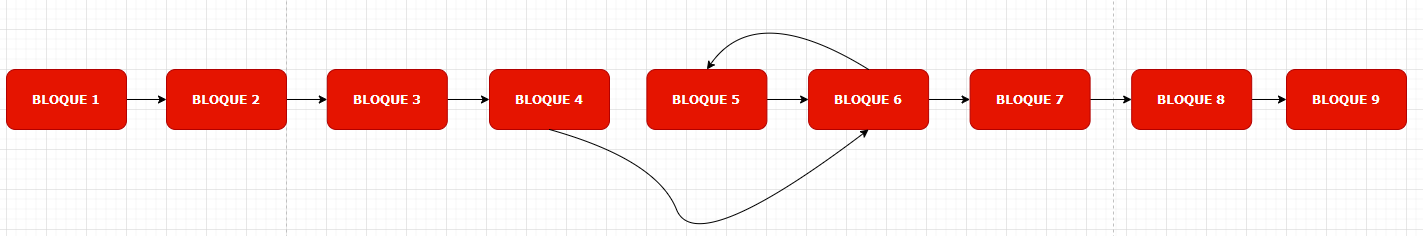
\includegraphics[scale=0.5]{./imagenes/diagrama bloque}
    \caption{Diagrama de flujo de los bloques}
\end{figure}
\section{¿Existe alguna estructura de control? Indica qué basic blocks intervienen en ella.}
Se observa que los bloques $B_4$, $B_5$ y $B_6$ forman una estructura de control basada en el condicional del bloque 6.

Esta condición, en caso de cumplirse, realiza un salto a +71, que es el inicio del bloque 5 y tras recorrerse los bloques 5 y 6, se vuelve a comprobar la condición. Si esta vez no se cumple, proseguirá por el bloque 7 (o volverá a entrar en el bucle.).

Esta estructura, puede ser tanto de un bucle \textit{FOR} como de un bucle \textit{WHILE}, aparentemente. Pues en primer lugar se produce el salto y establece las condiciones (salto del bloque 4 al bloque 6, donde esta la condición) y luego se tienen en cuenta las condiciones.

\newpage
\section{Convertir el código completo de la función en código C.}
El código en C será:
\begin{verbatim}
#include <stdio.h>
#include <string.h>


int main(int argc, char *argv[]) {
  int valor = 0;
  char* cadena = "3jd9cjfk98hnd";
  int longitud = strlen(cadena);

  for (int i = 0; i < longitud; i++) {
    valor += cadena[i] * longitud;
  }
  
  printf("[+] Codigo generado: %i\n", valor);
} 
\end{verbatim}

Vamos a explicar a continuación cómo hemos obtenido este código: (NOTA: Pese a que en el código original de las líneas anteriores aparezca * al lado de char, es por un fallo del editor \LaTeX, nos referimos a $^{*}$)

En primer lugar, vemos que se usan las funciones \textit{printf} y \textit{sterlen}, que muestran el resultado por pantalla y calculan la longitud de una cadena, respectivamente, por tanto es necesario incluir \textit{stdio.h} y \textit{string.h}. 

A continuación, empezamos la construcción de la función main(), tenienod en cuenta los parámetros \textit{argc} y \textit{argv}. Podemos ver que en la posición +29 se prepara el valor 0x0, que es el 0, en [ebp-0x10], que se usa después en +89 y +107. En +89, se usa la instrucción \textit{add}, por tanto se está haciendo una suma al valor ya existente en la dirección indicada, y como +107 es la última antes de la función \textit{printf} (tras cargar la cadena de texto “[+] Codigo generado: \% i\textbackslash n"). 

Vemos ahora que la variable que contiene el valor inicial 0, contiene también el valor final que aparece por pantalla: podemos iniciar una variable int con valor 0. 

\begin{center}
int valor $= 0$;
\end{center}

Seguidamente, observamos que se carga la cadena de texto "3jd9cjfk98hnd" en  [ebp-0x14], y se usa como parámetro en la función \textit{strlen}, como podemos ver en
\begin{verbatim}
0x00000571 <+36>: lea eax,[ebx-0x19a0] ; “3jd9cjfk98hnd”
0x00000577 <+42>: mov DWORD PTR [ebp-0x14],eax
0x0000057d <+48>: push DWORD PTR [ebp-0x14]
0x00000580 <+51>: call 0x3e0 <strlen@plt>
\end{verbatim}
Además, el resultado de \textit{strlen} está almacenado en [epb-0x18], por tanto es necesario crear una variable para almacenarlo. 
\begin{center}
char$^{*}$ cadena $=$ "3jd9cjfk98hnd";\\
int longitud $=$ strlen(cadena);
\end{center}

Entramos ahora con las condiciones del bucle. Tras almacenar el valor 0 en [ebp-0xc] se produce un salto a +96, que es el comienzo de la comprobación del bucle. Esta comprobación, se hace entre [ebp-0x18] y [ebp-0xc], la longitud de la cadena de texto y la variable de control, respectivamente. Podemos deducir que la condición paraque el bucle avance es que la variable de control sea menor en valor a la de la longitud de texto. Esto lo podemos observar en +102
\begin{verbatim}
    0x000005b3 <+102>: jl 0x594 <main+71>
\end{verbatim}
Pues \textit{jl} se refiere a jump if less. 

Como último paso, vemos que aumenta en uno el valor almacenado en [ebp-0xc]. 
\begin{verbatim}
    0x000005a9 <+92>: add DWORD PTR [ebp-0xc],0x1
\end{verbatim}
Lo cual nos da pie el código:
\begin{center}
for (int i $=$ 0; i $<$ longitud; i$++$)
\end{center}

El grosso de la operación viene a continuación. Entre +71 y +82 se obtiene un carácter en específico de nuestra cadena. Este valor, se multiplica por la longitud de la cadena (que estaba almacenada en [ebp-0x18]) siendo almacenado el resultado en el registro eax, y sumándose a la variable de resultado [ebp-0x10] (como se puede ver en +85 y +89). 
\begin{center}
   valor $+=$ cadena[i] * longitud;
\end{center}

Por último, finalizado el bucle se carga "[+] Codigo generado: \% i\textbackslash n" y  se usa con la variable almacenada en [ebp-0x10] para mostrar su valor por pantalla, siendo parámetros de \textit{printf}. De donde obtenemos:

\begin{center}
   printf("[+] Codigo generado: \% i\textbackslash n", valor)
\end{center}

\section{Compilar el código generado e indicar el código resultante tras su ejecución. Compilar en 32bits agregando la opción –m32r.}
Si compilamos como se nos dice, obtenemos:
\begin{figure}[h]
    \centering
    \includegraphics[scale=1]{./imagenes/captura}
    \caption{Resultado del código}
\end{figure}

\section{Modificar el código fuente en C, para que genere un nuevo código a partir de otra cadena dada.}
Se nos solicita que modifiquemos el valor de la cadena en +36, es decir, de:
\begin{verbatim}
    0x00000571 <+36>: lea eax,[ebx-0x19a0] ; “3jd9cjfk98hnd”
\end{verbatim}
Por tanto solo tendremos que cambiar “3jd9cjfk98hnd” por “Congratulations!”, obteniendo el código:
\begin{verbatim}
#include <stdio.h>
#include <string.h>


int main(int argc, char *argv[]) {
  int valor = 0;
  char* cadena = "“Congratulations!”;
  int longitud = strlen(cadena);

  for (int i = 0; i < longitud; i++) {
    valor += cadena[i] * longitud;
  }
  
  printf("[+] Codigo generado: %i\n", valor);
} 
\end{verbatim}
que da como resultado: 26080.

\end{document} 
